% https://www.overleaf.com/project/new/template/19345?id=65231945&templateName=An+example+of+the+beamer+package&latexEngine=&texImage=texlive-full%3A2020.1&mainFile=
% https://www.overleaf.com/learn/latex/Beamer#Further_reading
\documentclass{beamer}
\addtobeamertemplate{navigation symbols}{}{%
    \usebeamerfont{footline}%
    % \setbeamerfont{footline}{series=\bfseries}
    % \usebeamercolor[fg]{footline}%
    % \setbeamercolor{footline}{fg=blue}
    \hspace{1em}%
    \raisebox{1.3pt}{\insertframenumber/\inserttotalframenumber}
}
\usepackage[UTF8]{ctex}
\setCJKsansfont[BoldFont=NotoSansSC-Bold.otf]{NotoSansSC-Regular.otf}
\usepackage{outlines}
\usepackage{subfigure}
\usepackage{bbm}
% \usepackage[utf8]{inputenc}
% \usepackage{CJKutf8}
\usetheme{Berkeley}
\usecolortheme{seahorse}

%------------------------------------------------------------
%This block of code defines the information to appear in the
%Title page
\title[RL x Quantum] %optional
{基于强化学习的量子电路综合}

\subtitle{开题报告}

\author[] % (optional)
{彭晋钧\inst{1}}

\institute[VFU] % (optional)
{
  \inst{1}%
  计算机科学与技术系\\
  清华大学\\
  \vspace{1em}
  指导教师:韩文弢\\
  校外指导:Zhihao Jia (CMU)
}

\date[2023] % (optional)
{本科生综合论文训练, 2023}

%End of title page configuration block
%------------------------------------------------------------

%------------------------------------------------------------
%The next block of commands puts the table of contents at the 
%beginning of each section and highlights the current section:

\AtBeginSection[]
{
  \begin{frame}
    \frametitle{Table of Contents}
    \tableofcontents[currentsection]
  \end{frame}
}
%------------------------------------------------------------

\begin{document}
% \begin{CJK}{UTF8}{gbsn}

%The next statement creates the title page.
\frame{\titlepage}


%---------------------------------------------------------
%This block of code is for the table of contents after
%the title page
\begin{frame}
\frametitle{Table of Contents}
\tableofcontents
\end{frame}
%---------------------------------------------------------

\section{Background}

\subsection{Quantum Circuit}
\begin{frame}{Background - Quantum Circuits}
    \begin{columns}
        \column{0.6\textwidth}
            \begin{outline}
                \1 Qubit; State vector
                \1 Quantum gate $\leftrightarrow$ Unitary matrix
                    \2 single-qubit gate
                    \2 two-qubit gate
                \1 Gate set: a set of specific gates
                \1 Quantum circuit
                    \2 Logical qubit
                    \2 Mapping to physical qubit
            \end{outline}
            \vspace{1em}
            \begingroup
                \small
                $$
                \left(\begin{array}{llll}
                0 & 1 & & \\
                1 & 0 & & \\
                & & 0 & 1 \\
                & & 1 & 0
                \end{array}\right)\left(\begin{array}{l}
                v_{00} \\
                v_{01} \\
                v_{10} \\
                v_{11}
                \end{array}\right)
                $$
            \endgroup
        \column{0.4\textwidth}
            \begin{figure}
                \centering
                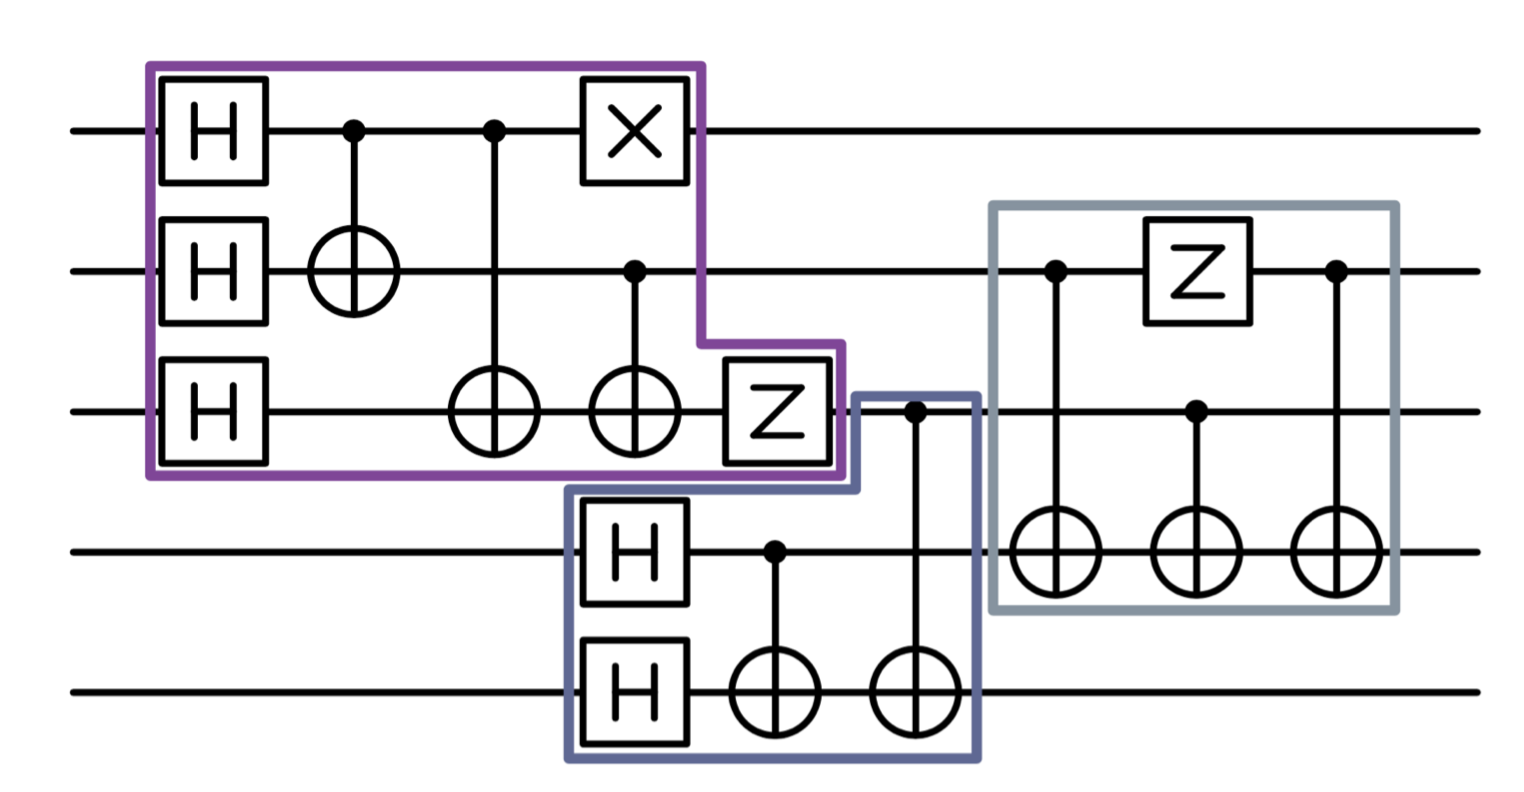
\includegraphics[scale=0.08]{qc.png}
            \end{figure}
            \begin{figure}
                \centering
                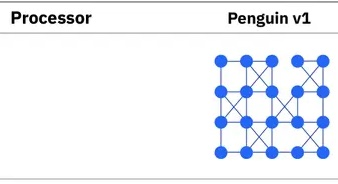
\includegraphics[scale=0.32]{IBM_penguin.jpg}
            \end{figure}
    \end{columns}
\end{frame}

\subsection{Quantum Circuit Optimization}
\begin{frame}{Background - QCO}
    \begin{outline}
        \1 Quantum Circuit Optimization: reduce gate count/CNOT count/depth...
        \1 Qubit Mapping/Routing: SWAP insertion increases \#gates
        \1 End-to-end optimization: topology-aware synthesis
            \2 given target unitary matrix
            \2 start from an empty circuit
            \2 insert executable gates
            \2 stop when reaching around the target
    \end{outline}
    \begin{figure}
        \centering
        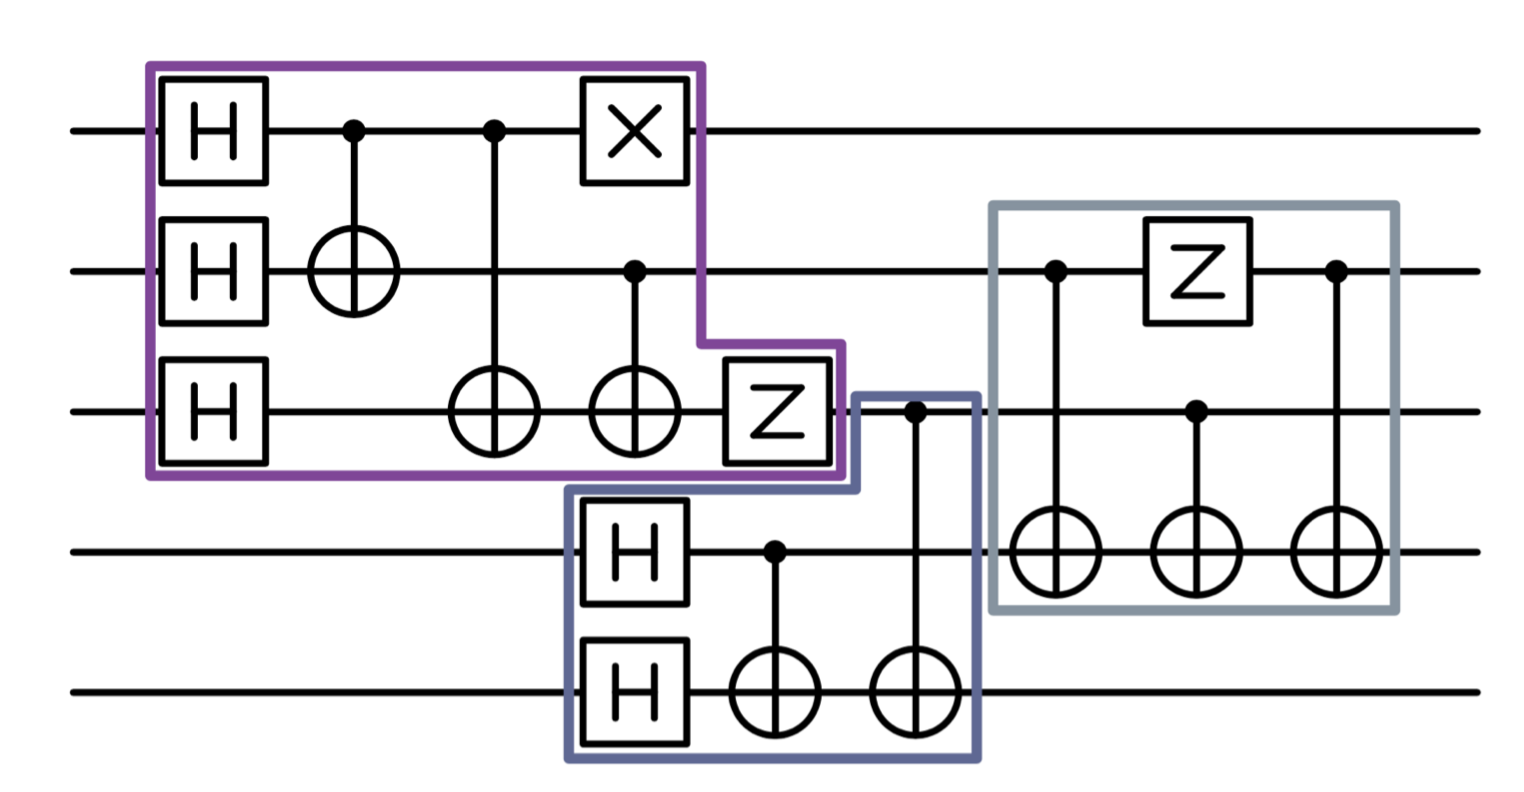
\includegraphics[scale=0.08]{qc.png}
    \end{figure}
\end{frame}

\section{Existing Works}

\begin{frame}{Existing Works}
    \begin{outline}
        \1 QSearch/LEAP: A* tree search for small circuits
            \2 \#qubits $\leq$ 6
            \2 reduce CNOT count \& depth
            \2 where to insert CNOT at each step
        \1 TopAS
            \2 Partitioning: wide circuits $\rightarrow$ small circuits (\#qubits $\leq$ 6)
            \2 Subtopology selection with a similarity function
            \2 Local synthesis with subtopology awareness
            \2 Partition replacement \& Final mapping
        \1 RL-assisted synthesis for single-qubit circuits
            \2 Moro et al. (2020), Zhang et al. (2020)
            \2 given a (native) gate set
            \2 decompose a target matrix into a sequence of gates
            \2 let RL agent decide which gate to insert at each step
        % Solovay–Kitaev theorem
    \end{outline}
\end{frame}

\section{Opportunities}
\begin{frame}{Opportunities}
    \begin{outline}
        \1 Improve QSearch/LEAP
        % Table 5 of LEAP: TFIM-10: 5 qubits, 11320.8
            \2 Distance estimation
                \3 data-driven linear regression based on $D(U, U_{\text{target}})$ $\rightarrow$ value network
            \2 Policy
                \3 select the node having min distance to the target $\rightarrow$ policy network
            \2 Reward for RL
                \3 constant negative value, e.g., -1
            \2 State encoding for RL
                \3 unitary matrix $\in \mathcal{M}_{2^n}(\mathbbm{C})$ remained to approximate
                \3 limitation: cannot scale to large n
                \3 design the network to handle some invariants
                % TODO attention like network; q, k, U, v
                % current circuit v.s. target circuit -> output where to insert
            % \2 RL for single-qubit gate insertion % TODO meaningful??? U3 params tuning?
            % will the CNOT-U3 interleaving insertion leads to suboptimal?
        % TopAS: how to choose sub-topology?
    \end{outline}
\end{frame}

\section{Plan}
\begin{frame}{Plan}
    \begin{outline}
        \1 1: Run \& re-evaluate LEAP
        \1 2: Build RL pipeline
        \1 3 - 4: Evaluate and improve the algorithm
        % \1 4: Explore other gate sets
        \1 5: Summary \& writing
    \end{outline}
\end{frame}

\begin{frame}{The End}
    Thank you!    
\end{frame}

% \end{CJK}
\end{document}



\iffalse

%------------------------------------------------------------
%This block of code defines the information to appear in the
%Title page
\title[About Beamer] %optional
{About the Beamer class in presentation making}

\subtitle{A short story}

\author[Arthur, Doe] % (optional)
{A.~B.~Arthur\inst{1} \and J.~Doe\inst{2}}

\institute[VFU] % (optional)
{
  \inst{1}%
  Faculty of Physics\\
  Very Famous University
  \and
  \inst{2}%
  Faculty of Chemistry\\
  Very Famous University
}

\date[VLC 2021] % (optional)
{Very Large Conference, April 2021}

\logo{\includegraphics[height=1cm]{overleaf-logo}}

%End of title page configuration block
%------------------------------------------------------------

%------------------------------------------------------------
%The next block of commands puts the table of contents at the 
%beginning of each section and highlights the current section:

\AtBeginSection[]
{
  \begin{frame}
    \frametitle{Table of Contents}
    \tableofcontents[currentsection]
  \end{frame}
}
%------------------------------------------------------------


\begin{document}
\begin{CJK}{UTF8}{gbsn}

%The next statement creates the title page.
\frame{\titlepage}


%---------------------------------------------------------
%This block of code is for the table of contents after
%the title page
\begin{frame}
\frametitle{Table of Contents}
\tableofcontents
\end{frame}
%---------------------------------------------------------


\section{First section}

\subsection{Item}

\subsubsection{What?}

%---------------------------------------------------------
%Changing visivility of the text
\begin{frame}
\frametitle{Show item}
This is a text in second frame. For the sake of showing an example.

\begin{itemize}
    \item<1-> Text visible on slide 1
    \item<2-> Text visible on slide 2
    \item<3> Text visible on slides 3
    \item<4-> Text visible on slide 4
\end{itemize}
\end{frame}

%---------------------------------------------------------

\subsection{Pause}

%---------------------------------------------------------
%Example of the \pause command
\begin{frame}
\frametitle{Show pause}
In this slide \pause

the text will be partially visible \pause

And finally everything will be there
\end{frame}
%---------------------------------------------------------

\subsection{Pause2}

%---------------------------------------------------------
%Example of the \pause command
\begin{frame}
\frametitle{Show pause 2}
In this slide \pause

the text will be partially visible \pause

And finally everything will be there
\end{frame}
%---------------------------------------------------------

\subsection{Pause3}

%---------------------------------------------------------
%Example of the \pause command
\begin{frame}
\frametitle{Show pause 3}
In this slide \pause

the text will be partially visible \pause

And finally everything will be there
\end{frame}
%---------------------------------------------------------

\section{Second section}

%---------------------------------------------------------
%Highlighting text
\begin{frame}
\frametitle{Sample frame title}

In this slide, some important text will be
\alert{highlighted} because it's important.
Please, don't abuse it.

\begin{block}{Remark}
Sample text
\end{block}

\begin{alertblock}{Important theorem}
Sample text in red box
\end{alertblock}

\begin{examples}
Sample text in green box. The title of the block is ``Examples".
\end{examples}
\end{frame}
%---------------------------------------------------------


%---------------------------------------------------------
%Two columns
\begin{frame}
\frametitle{Two-column slide}

\begin{columns}

\column{0.5\textwidth}
This is a text in first column.
$$E=mc^2$$
\begin{itemize}
\item First item
\item Second item
\end{itemize}

\column{0.5\textwidth}
This text will be in the second column
and on a second tought this is a nice looking
layout in some cases.
\end{columns}
\end{frame}
%---------------------------------------------------------

\end{CJK}
\end{document}

\fi
